% 第十一届湖南省研究生数学建模竞赛 B 题论文
% 版式对齐：competition_question/（必读）第十一届湖南省研究生数学建模竞赛论文格式规范.docx
% 匿名：无队号、单位、姓名；页眉空白（规范禁止页眉出现队号）；页脚中部页码自 1
% 编译：bash compile.sh  或  xelatex main.tex （两次）
\documentclass[UTF8,a4paper,zihao=-4,fontset=fandol]{ctexart}

% 页边距取规范 Word 的上下 2.54cm，左右按惯例不少于 2.5cm
\usepackage[a4paper,top=2.54cm,bottom=2.54cm,left=2.54cm,right=2.54cm]{geometry}
\usepackage{amsmath,amssymb,bm}
\usepackage{booktabs,tabularx,multirow,makecell}
\usepackage{graphicx}
\usepackage{float}
\usepackage{tikz}
\usetikzlibrary{arrows.meta,positioning}
\usepackage{caption}
\usepackage{setspace}
\usepackage{enumitem}
\usepackage{xcolor}
\usepackage{fancyhdr}
\usepackage[hidelinks]{hyperref}
\usepackage{listings}

% 正文英文：Times 同类（本机无 Times New Roman 时用 TeX Gyre Termes）
\setmainfont{TeX Gyre Termes}[
  Extension      = .otf,
  UprightFont    = texgyretermes-regular,
  BoldFont       = texgyretermes-bold,
  ItalicFont     = texgyretermes-italic,
  BoldItalicFont = texgyretermes-bolditalic,
  Path           = /usr/share/texmf/fonts/opentype/public/tex-gyre/,
  Ligatures      = TeX,
]

\hypersetup{pdftitle={考虑送端碳排不确定性的区域电网鲁棒碳流追踪与低碳调度},pdfauthor={},pdfcreator={}}


% 题目三号黑体居中；一级小三黑左齐；二级四号黑左齐；三级小四黑左齐（均加粗、不居中）
\ctexset{
  section/format = \heiti\zihao{-3}\bfseries\raggedright,
  section/beforeskip = 0.7ex plus .2ex,
  section/afterskip = 0.45ex plus .1ex,
  subsection/format = \heiti\zihao{4}\bfseries\raggedright,
  subsection/beforeskip = 0.55ex plus .2ex,
  subsection/afterskip = 0.35ex plus .1ex,
  subsubsection/format = \heiti\zihao{-4}\bfseries\raggedright,
  subsubsection/beforeskip = 0.4ex plus .1ex,
  subsubsection/afterskip = 0.25ex,
}
% 正文小四宋体、单倍行距、段前段后 0.25 行、首行缩进 2 字符
\setstretch{1.0}
\setlength{\parskip}{0.25\baselineskip}
\setlength{\parindent}{2em}
\setlist{nosep,leftmargin=2em}

% 图注、表头：楷体 11 号
\DeclareCaptionFont{kai11}{\kaishu\fontsize{11pt}{15pt}\selectfont}
\captionsetup{font=kai11,labelsep=quad,skip=4pt}
\captionsetup[table]{position=top,skip=3pt}
\captionsetup[figure]{position=bottom,skip=3pt}

\renewcommand{\thefigure}{\arabic{figure}}
\renewcommand{\thetable}{\arabic{table}}
\renewcommand{\theequation}{\arabic{equation}}

% 页眉空白；页脚中部阿拉伯页码
\pagestyle{fancy}
\fancyhf{}
\fancyfoot[C]{\thepage}
\renewcommand{\headrulewidth}{0pt}
\renewcommand{\footrulewidth}{0pt}
\fancypagestyle{plain}{%
  \fancyhf{}%
  \fancyfoot[C]{\thepage}%
  \renewcommand{\headrulewidth}{0pt}%
}

\lstset{
  basicstyle=\ttfamily\zihao{6},
  language=Python,
  breaklines=true,
  columns=fullflexible,
  frame=single,
  rulecolor=\color{black!25},
  aboveskip=4pt,
  belowskip=4pt,
  showstringspaces=false,
  keywordstyle=\bfseries,
  commentstyle=\normalfont,
}

\begin{document}

% 第 1 页：竞赛名（对齐规范 Word 题头）+ 论文题目 + 摘要 + 关键词
\begin{center}
{\heiti\zihao{-2}\bfseries 第十一届湖南省研究生数学建模竞赛}\\[1.4em]
{\heiti\zihao{3}\bfseries 考虑送端碳排不确定性的区域电网}\\[0.35em]
{\heiti\zihao{3}\bfseries 鲁棒碳流追踪与低碳调度}
\end{center}
\vspace{1.1em}

\noindent{\heiti\zihao{-4}\bfseries 摘\quad 要}\quad
针对某省八区域电网的多源计量口径差异、跨区碳责任划分、五年项目约束耦合及省外送端碳因子波动，本文构建由数据调和、碳流追踪、项目组合和不确定性分析组成的模型链，全部计算均可由程序复现。问题一在守恒约束下进行标准化 Huber 数据调和，并将年度工程线损作为软先验。23 项异常仅作诊断标记，稳健目标为 291.0288，最大平衡残差为 $4.89\times10^{-13}$\,GWh，E05 线损估计为 0.01675。问题二逐月求解比例共享碳势，并通过 500 次条件参数自举传播量测误差。每次自举均先生成伪观测，再完整执行调和与碳流计算。A4、A5 年均碳强度分别为 0.62399、0.15217\,kgCO$_2$/kWh，A4$\to$A3 碳流点估计为 4366.34\,kt，95\% 条件区间为 $[4356.76,4419.04]$\,kt。$\lambda=0.5$ 与所构造的 Shapley 分配一致，但这来自特征函数的结构恒等式，不能单独证明该权重在政策上最公平。问题三按缺供、投资和最大相对区域超额建立词典序 $\varepsilon$-约束。最低投资 $C^*=964.970$ 百万元；推荐 $\varepsilon=1\%$，对应投资 974.603 百万元，加权基线的最大相对超额由 8.281\% 降至 7.611\%，全部硬约束均通过独立回代。问题四分别检验设计集与统一 $\Gamma$ 集，并区分软违约和硬可行。完整 $\Gamma=1$ 下的最小不可避免缺口为 14.8488\,kt，最大硬可行半径 $\tau^*=0.953003$；四条无概率典型路径的非预见最小最大相对遗憾为 141.595\%，且均满足硬约束。滚动比较采用同一状态下的剩余期目标，2028、2029 年分别改善 307.566、434.874 百万元。该改善包含避免的违约罚，不能等同于投资节省。

\vspace{0.6em}
\noindent{\heiti\zihao{-4}\bfseries 关键词：}\ 数据调和；碳排放流；责任共担；项目组合优化；预算鲁棒优化

\newpage

\section{问题重述}

某省一次能源供给不足，部分用电依赖省外输入。省内八个区域（记为 $A1,\ldots,A8$）的产业结构、电源构成和发展阶段差异较大，并通过 11 条输电通道相连。由于各类电源的碳强度不同，仅按本地发电核算难以反映跨区用电的碳责任。2026至2030 年计划滚动实施 35 个候选项目，涉及工业节能、建筑改造、交通电气化、分布式光伏和通道升级。项目之间同时存在资源竞争、互斥关系和协同效应。省外送端电源结构还会随季节及供需变化，使输入电碳因子具有不确定性。

附件给出 2025 年分月监测、年度汇总、通道工程参数、排放因子、五年双控约束、项目库以及送端碳因子区间与情景。数据来自不同监测系统，存在缺失、口径差与个别物理上不合理的记录。题面能量平衡为
\begin{equation}
G_{i,t}+I_{i,t}+\sum_{j\neq i}T_{j,i,t}
=D_{i,t}+\sum_{j\neq i}T_{i,j,t}+L_{i,t},
\label{eq:balance}
\end{equation}
其中 $G$ 为本地发电，$I$ 为省外输入，$T$ 为区域间输电，$D$ 为终端用电，$L$ 为损耗；因测量误差，\eqref{eq:balance} 在原始数据上并不成立。电量单位为 GWh，与排放因子（kgCO$_2$/kWh）相乘得碳排放（ktCO$_2$）。

五个问题依次是：（1）识别并校正多源电量，估计通道损耗，评价观测影响度；（2）追踪碳流，给出逐月终端碳强度，并按发电地、用电地及兼顾二者的口径分担责任；（3）在供能与全省碳上限下安排五年项目，使综合成本合理，并检验方案稳定性；（4）评估送端碳因子不确定对问题三方案的冲击，给出仍可满足约束的调整机制并量化抗风险代价；（5）面向选定决策主体撰写约 1000 字咨询报告。附件 6 的题面文字写“突发事件”，Excel 给出的是碳因子上下界与情景 S0至S3，本文以 Excel 为准。

\section{问题分析与技术路线}

四个建模环节存在明确的前后依赖。碳势计算需要满足守恒的电量数据，五年碳约束依赖 2025 年区域碳强度，而不确定性分析则以问题三的基准方案为参照，衡量冲击幅度及相应的抗风险成本。

问题一采用过程系统中的稳健数据调和方法。在硬守恒约束下，以 Huber 损失校正冗余观测，再通过普通 WLS 和污染实验比较粗差对估计结果的影响。该模型与电力系统稳健状态估计具有相同结构，但状态变量改为区域月度电量及通道送、受端电量。

问题二将潮流追踪中的比例共享原则用于碳流核算。同一节点的各项出流具有相同碳势，碳量随到达电量在网络中传递。为估计条件量测区间，每个伪观测样本都重新经过完整的数据调和与碳流计算。责任核算包括生产侧、消费侧和线性共担三种口径，并以全省碳量守恒进行校验。

问题三建立多年期投资与运行耦合的 MILP。若以罚权同时处理缺供和区域超额，两类目标间的交换率取决于人为设定的权重。为避免这一问题，本文依次优化缺供、投资和最大相对区域超额，并扫描 $\varepsilon$。问题四以完整 $\Gamma$ 集确定压力下限，以无概率的 S0至S3 描述典型适应路径。前者用于计算硬可行半径和恢复边界，后者用于求解带非预见约束的最小最大遗憾。滚动分析仅比较同一决策时点的剩余期目标（objective-to-go）。

技术路线如图\ref{fig:roadmap}所示：附件 1/2 $\to$ 问题一调和 $\to$ 附件 3 与碳势方程 $\to$ 问题二责任与份额矩阵 $S_{ij}$ $\to$ 附件 4/5 的五年 MILP $\to$ 附件 6 的情景与 $\Gamma_t$ $\to$ 咨询报告。计算环境为 Python 3，二次规划使用 cvxpy/Clarabel，MILP 使用 Pyomo/HiGHS。所有数值均由程序生成并交叉核验，正文不作人工改写。

\begin{figure}[H]
\centering
\begin{tikzpicture}[node distance=0.65cm and 0.78cm, >=Latex,
  box/.style={draw, rounded corners=2pt, align=center, minimum height=1.15cm,
    text width=2.05cm, font=\small, fill=gray!8},
  arr/.style={->, line width=0.7pt}]
  \node[box, fill=blue!10] (d) {附件 1、2\\多源监测};
  \node[box, fill=green!12, right=of d] (q1) {问题一\\调和与线损};
  \node[box, fill=yellow!18, right=of q1] (q2) {问题二\\碳流与分担};
  \node[box, fill=red!10, below=of q2] (q3) {问题三\\五年项目 MILP};
  \node[box, fill=purple!10, left=of q3] (q4) {问题四\\鲁棒与滚动};
  \node[box, fill=cyan!12, left=of q4] (q5) {问题五\\决策咨询};
  \draw[arr] (d) -- (q1);
  \draw[arr] (q1) -- (q2);
  \draw[arr] (q2) -- (q3);
  \draw[arr] (q3) -- (q4);
  \draw[arr] (q4) -- (q5);
\end{tikzpicture}
\caption{五个问题的计算顺序。附件数据经问题一调和后进入碳流，再进入五年项目和鲁棒滚动。}
\label{fig:roadmap}
\end{figure}

\section{基本假设与符号}

\subsection{基本假设}

\begin{enumerate}[label=\textbf{H\arabic*.}]
\item 校正后的月度电量满足区域能量平衡；通道损耗落在线路上，入流按受端计量、出流按送端计量。
\item 区内输配损耗无直接关口，采用“终端用电 $\times 5\%$”作为可松弛先验，不将损耗率固定为 5\%。
\item 碳流采用比例共享与送端承担线损碳的主口径；节点碳势由入流碳量守恒唯一确定。
\item 2026至2030 年区域终端碳强度沿用 2025 年追踪结果，再用附件给出的 $\kappa_y$ 做全省强度调整；官方碳核算不显式依赖区域间潮流。
\item 问题四将 2025 年“省外输入分接入区”份额矩阵 $S_{ij}$ 固定至 2030 年。该假设较强，后文对其局限作定量分析。
\item 送端不确定性仅采用附件 6 给出的因子区间与情景，不额外假设突发事件时间线。
\item 项目效益自开工年加建设周期起生效；已开工规模在滚动中不可逆。
\item 主方案综合成本不折现，与附件年度投资上限同口径；8\% 折现仅作敏感性。
\end{enumerate}

\subsection{主要符号}

\begin{table}[htbp]
\centering
\caption{主要符号}
\label{tab:symbol}
\begin{tabular}{llp{7.6cm}}
\toprule
符号 & 单位 & 含义 \\
\midrule
$i,j$ & 无量纲 & 区域，$i,j\in\{A1,\ldots,A8\}$ \\
$t,y$ & 无量纲 & 月份（2025）或规划年（2026至2030） \\
$x_k,\hat x_k,\sigma_k$ & GWh & 观测、校正值、不确定度 \\
$\eta_e$ & 无量纲 & 通道 $e$ 损耗率 \\
$\rho_{i,t}$ & kgCO$_2$/kWh & 节点碳势（终端用电碳强度） \\
$P^+_i,C^+_i$ & ktCO$_2$ & 扩展生产责任、全口径消费责任 \\
$F_{j\to i}$ & ktCO$_2$ & 通道 $j\to i$ 到达电量携带的碳 \\
$S_{ij}$ & 无量纲 & 区域 $i$ 消费中来自接入区 $j$ 省外输入的份额 \\
$E_{i,y}$ & ktCO$_2$ & 规划年消费侧碳排放 \\
$\overline E_y$ & ktCO$_2$ & 全省消费侧碳上限 \\
$B_{i,y}$ & ktCO$_2$ & 区域软预算 \\
$w_y$ & 无量纲 & 预算惯性权重（0.85$\to$0.65） \\
$\xi_{j,y}$ & 无量纲 & 送端因子相对基准的乘数 \\
$\Gamma_y$ & 无量纲 & 年份 $y$ 的不确定预算 \\
$C^*,\varepsilon$ & 百万元，无量纲 & 零缺供最低投资及其投资容许比例 \\
$R$ & 无量纲 & 最大区域相对预算超额 \\
$\tau$ & 无量纲 & $\Gamma$ 的缩放系数（硬可行半径参数） \\
\bottomrule
\end{tabular}
\end{table}

\section{问题一：多源电量一致性校正}

\subsection{异常识别}

求解调和模型前，先进行不依赖优化器的结构性校验。检查内容包括分部门用电与终端用电的加总关系、月度累加与年度汇总的一致性、通道隐含损耗与工程值的偏差、受端电量是否超过送端电量、容量是否越限，以及按 5\% 终端用电补入缺失区内损耗后的能量平衡标准化残差。以 $|z|>3$ 为粗差阈值，共标记 23 条记录。最严重的是 2025-09 区域 A2，平衡残差为 $z=32.5$，同时缺失该月工业用电和终端用电合计。通道 E03 在 8 月的隐含损耗率为 0.175，远高于工程值 0.025。E10 年度汇总受端电量为 1563.8\,GWh，超过送端电量 1559.6\,GWh。月度与年度两套系统对 A2 工业用电的记录相差 8.71\%。四处月度空值（A7 风电、A4 水电、A2 工业与终端合计）在模型中作为自由变量。

\subsection{守恒约束下的标准化 Huber 调和}

记 $\boldsymbol y$ 为全部待校正量（分源发电、省外输入、分部门用电、通道送/受端电量），$z_k$ 为观测，$h_k(\boldsymbol y)$ 为对应状态量。对观测残差使用阈值 $\delta=1.5$ 的标准化 Huber 损失，对区内损耗与年度工程线损使用二次软先验\cite{Crowe1996data,Narasimhan1999data}：
\begin{equation}
\min_{\boldsymbol y,\boldsymbol L}
\sum_{k\in\mathcal O}\phi_{1.5}\!\left(
\frac{h_k(\boldsymbol y)-z_k}{\sigma_k}\right)
+\sum_{i,t}\left(\frac{L_{i,t}-0.05D^{\rm obs}_{i,t}}
{\sigma^L_{i,t}}\right)^2
+\sum_{e\in\mathcal E_+}\left[
\frac{\sum_t r_{e,t}-(1-\eta_e^{\rm eng})\sum_t s_{e,t}}
{\sigma^{\eta}_e}\right]^2,
\label{eq:wls}
\end{equation}
其中 $\phi_\delta(u)=u^2$（$|u|\le\delta$），否则为 $2\delta|u|-\delta^2$；$\mathcal E_+$ 是有有效流量的通道集合，$s,r$ 分别为送、受端电量。$\sigma_k=\max(\mathrm{rel}_k|z_k|,\underline\sigma_k)$，发电/输入/分项用电取 2\%，终端合计与年度汇总取 1.5\%，通道计量取 2.5\%。约束为逐区域逐月能量平衡\eqref{eq:balance}、$0\le r\le s\le$ 月度容量、非负性和结构性零流量。式\eqref{eq:wls}中的表达均为线性项或凸分段二次项，因此一次求解即可，无须将估计得到的 $\eta$ 按固定轮数反复回代。求解后按 $\hat\eta_e=1-\sum_t\hat r_{e,t}/\sum_t\hat s_{e,t}$ 统计年度线损。E07 全年无有效流量，无法由数据识别，故保留工程值 0.027。该模型是广义状态估计的稳健版本\cite{Schweppe1970power,Abur2004power,Liu2023robust}，区内 5\% 损耗与工程线损仅作为收缩先验。物理约束调和后再追踪排放的方法亦见文献\cite{deChalendar2021physics}。

上述 23 项原始异常和口径不一致仅作为诊断标记，不能直接认定为粗差。影响度计算对候选观测施加对称 $\pm5\%$ 有限差分，基准解与扰动解均采用同一 Huber 模型。区域年度用电变化和线损率变化先分别标准化，再合成为无量纲分数，因而不会直接混合 GWh 与线损率，结果也不受人为迭代轮数影响。

\subsection{校正结果}

\begin{sloppypar}
Huber 模型达到最优，稳健目标为 291.028826。标准化观测残差平方和为 102.071576，除以 1274 个观测项得到 0.08011898。该值只是描述性 $\mathrm{RSS}/n$：模型另含 106 个先验残差、硬约束、相关观测与估计状态，不宜当作约化卡方，也不宜据此做拟合优度检验。平衡残差最大 $4.89\times10^{-13}$\,GWh，容量、非负性、$r\le s$ 与结构性零流量均满足。四处缺失插补为 48.15、68.73、493.62、881.32\,GWh（依次为 A7 风电、A4 水电、A2 工业、A2 终端）；全省区内损耗率为 1.742\%。E05 年度线损为 0.01675（工程值 0.02000），E10 为 0.02777。影响度前三依次是 E10 年度送端汇总、E10 年度受端汇总和 2025-08 A4 省外输入，建议优先复核年度/月度关口口径。
\end{sloppypar}

\begin{figure}[H]
\centering
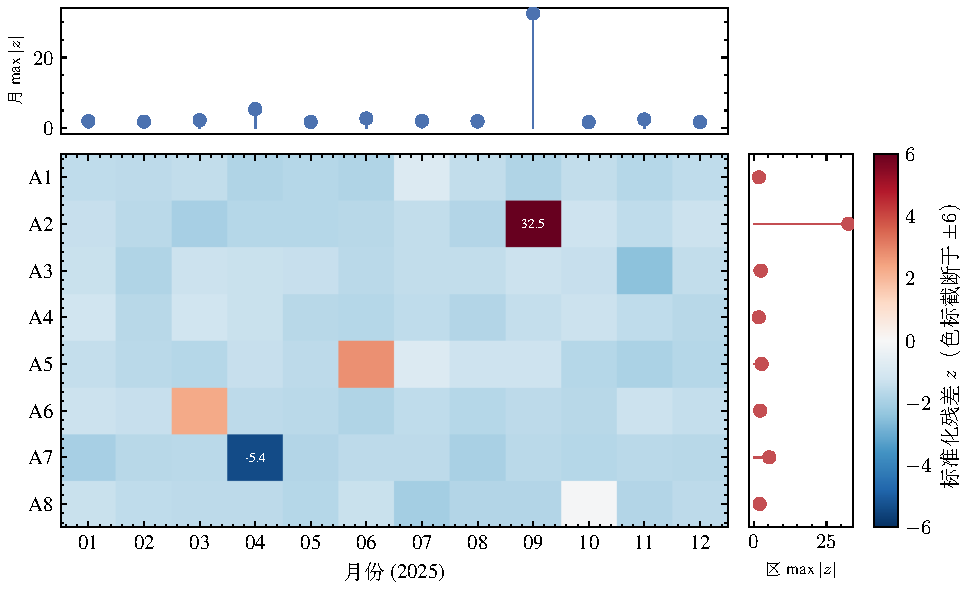
\includegraphics[width=0.92\textwidth]{../src/outputs/q1/fig_q1_raw_residual_heatmap.pdf}
\caption{校正前各区域逐月能量平衡标准化残差及边际统计。色标截断于 $\pm 6$，格内标注 $|z|>3$；上缘与右侧分别给出各月、各区的 $\max|z|$，A2 九月的极端值 $z=32.5$ 另以数值标明。}
\label{fig:q1res}
\end{figure}

\begin{figure}[H]
\centering
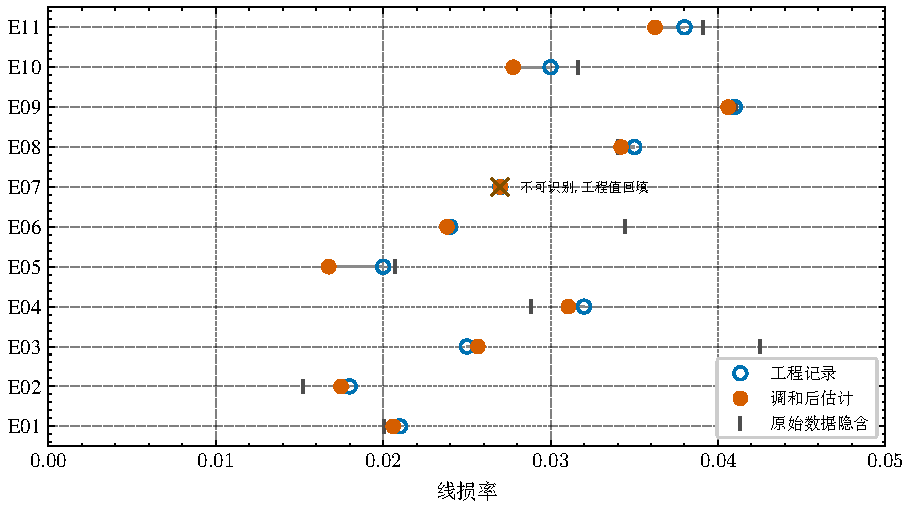
\includegraphics[width=0.88\textwidth]{../src/outputs/q1/fig_q1_eta_compare.pdf}
\caption{通道线损率比较。空心点为工程记录，实心点为调和估计，竖线为原始隐含损耗率。E05 工程值高于估计值，E03 的偏高隐含损耗率经调和后降低，E07 因无有效流量而保留工程值。}
\label{fig:eta}
\end{figure}

对称扰动后的影响分数见图\ref{fig:influence}。E10 年度送、受端汇总的影响分数最高，其次为 A4 八月省外输入，说明跨口径关口总量对全网估计结果最敏感。

\begin{figure}[H]
\centering
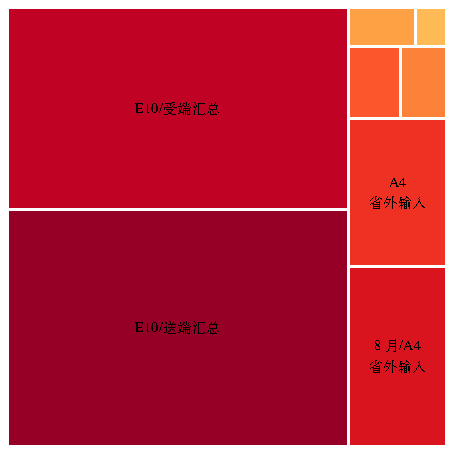
\includegraphics[width=0.88\textwidth]{../src/outputs/q1/fig_q1_influence.pdf}
\caption{关键观测在对称 $\pm 5\%$ 扰动下的综合影响分数。矩形面积正比于影响分数，其中 E10 年度送、受端汇总所占面积最大。}
\label{fig:influence}
\end{figure}

\begin{table}[htbp]
\centering
\caption{Huber 与 WLS 的清洁数据一致性及污染稳健性}
\label{tab:q1sens}
\resizebox{\textwidth}{!}{\begin{tabular}{lccccc}
\toprule
方法 & 清洁 $\mathrm{RSS}/n$ & 状态差异 RMSE & 污染平均 RMSE & 用电最大变化 & 线损最大变化 \\
\midrule
Huber & 0.080119 & 0 & 0.038782 & 0.164\% & 0.00333 \\
WLS & 0.078737 & 0.003509 & 0.045085 & 0.313\% & 0.00528 \\
\bottomrule
\end{tabular}}
\end{table}

在清洁数据上，两种方法的状态归一化 RMSE 为 0.003509，说明稳健化没有明显改变正常观测下的估计结果。六类确定性污染实验中，WLS 与 Huber 的平均状态 RMSE 之比为 1.1625，且 WLS 的年度用电与线损最大变化均较大。因此，本文依据污染条件下的稳定性选择 Huber，而不是依据清洁数据上的 $\mathrm{RSS}/n$，后者由 WLS 略占优势。

\section{问题二：碳流追踪与责任分担}

\subsection{节点碳势}

在校正后的电量网络上，设节点 $i$ 的总入流能量为 $Q_i$（本地四类电源 + 省外输入 + 通道到达电量）。比例共享假定：节点一旦混合，所有出流（负荷、损耗、外送）携带同一碳势 $\rho_i$\cite{Bialek1996tracing,Kang2015carbon}。以送端承担通道损耗碳为主口径，到达受端的电量只携带送端碳势，损耗碳留在送端台账。碳势满足
\begin{equation}
\bigl(\mathrm{diag}(\boldsymbol Q)-\boldsymbol C\bigr)\boldsymbol\rho=\boldsymbol b,
\label{eq:rho}
\end{equation}
其中 $C_{ij}$ 为 $j\to i$ 到达电量，$b_i$ 为节点 $i$ 本地发电与省外输入注入的碳量。\eqref{eq:rho} 逐月为 $8\times 8$ 线性方程组。来源份额由同一比例共享结构、以各类注入能量为右端项一次解出，不再把份额额外除以 $Q_i$。省外输入按接入区分列的份额矩阵 $S_{ij}$ 供问题四使用。

\subsection{三种责任口径与 Shapley}

扩展生产责任 $P^+_i$ 为本地发电碳加该区接入的省外输入碳\cite{Peters2008production}。全口径消费责任 $C^+_i$ 为终端用电碳加区内损耗碳及送端承担的通道损耗碳\cite{Davis2010consumption}。线性共担\cite{Gallego2005consistent,Lenzen2007shared}
\begin{equation}
R_i(\lambda)=\lambda P^+_i+(1-\lambda)C^+_i,\qquad \lambda\in\{0.3,0.5,0.7\}.
\label{eq:lambda}
\end{equation}
因 $\sum P^+=\sum C^+$，任意 $\lambda$ 下全省总量守恒。另构造通道碳转移博弈：记 $F_{j\to i}$ 为到达电量乘送端碳势，
\begin{equation}
v(S)=\sum_{i\in S}P^+_i+\sum_{j\notin S,\,i\in S}F_{j\to i}.
\label{eq:shapley}
\end{equation}
八个区域共有 $2^8=256$ 个联盟，可精确枚举 Shapley 值 $\varphi_i$\cite{Qin2020cooperative}。该特征函数将每条跨区转移的边际量平均分配给送、受两端，因此 $\varphi_i=(P_i^++C_i^+)/2$ 是结构恒等式，数值上与 $\lambda=0.5$ 一致（两位小数下个别 0.01\,kt 的差异来自舍入）。本文将其称为“五五共担的 Shapley 表示”。这一结果只适用于式\eqref{eq:shapley}定义的特征函数，不能据此判定 $\lambda=0.5$ 是政策上唯一的公平权重。

\subsection{追踪结果}

2025 年全省生产口径与消费全口径排放均为 35883.78\,kt，未舍入责任守恒误差为 0（CSV 按两位小数汇总时相差 0.01\,kt）。终端碳强度以 A4 最高（0.62399）、A5 最低（0.15217）。图\ref{fig:rho}呈现两类季节特征：A1、A3、A4、A6 全年保持高位，A5、A7、A8 在夏季下降。A3 的消费责任为 5435.60\,kt，是扩展生产责任 1015.92\,kt 的 5.35 倍；其消费电量中省外输入占 48.45\%，其中 46.96 个百分点经 A4 接入。主路径 A4$\to$A3 的点估计为 4366.34\,kt，其次为 A4$\to$A2 的 969.19\,kt 和 A6$\to$A8 的 777.98\,kt。这一结果与省内“碳外包”格局一致\cite{Feng2013outsourcing}。生产侧口径会低估受电区责任，消费侧口径则无法体现送端枢纽的生产责任。本文以 $\lambda=0.5$ 作为协商基准，同时报告 0.3 和 0.7 两种权重下的结果。

\begin{figure}[H]
\centering
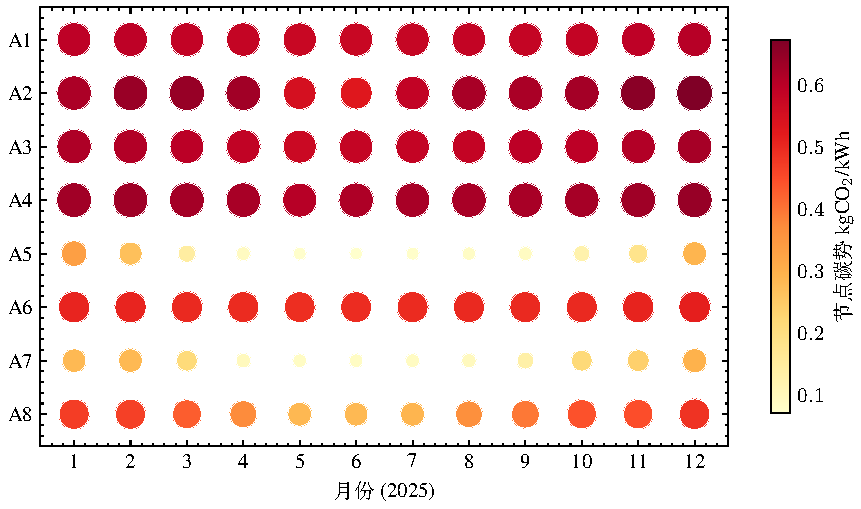
\includegraphics[width=0.92\textwidth]{../src/outputs/q2/fig_q2_rho_monthly.pdf}
\caption{各区域 2025 年逐月节点碳势气泡矩阵（送端承担口径）。圆面积与颜色表示碳势；A1至A4、A6 全年高位，A5、A7、A8 夏季气泡明显缩小。}
\label{fig:rho}
\end{figure}

图\ref{fig:originmix}给出强度差异的来源。A5、A7 的本地清洁电量占比分别为 82.35\% 和 78.48\%，其中水电分别为 72.68\% 和 56.52\%；两地碳势在丰水期（4至8 月）明显走低，年初和年末再回升。A1、A6 的省外输入占比分别为 69.44\% 和 71.27\%，其强度主要随接入电源结构变化。A2 火电占比 49.80\%，12 月碳势升至 0.67196，为八区最高单月。

\begin{figure}[H]
\centering
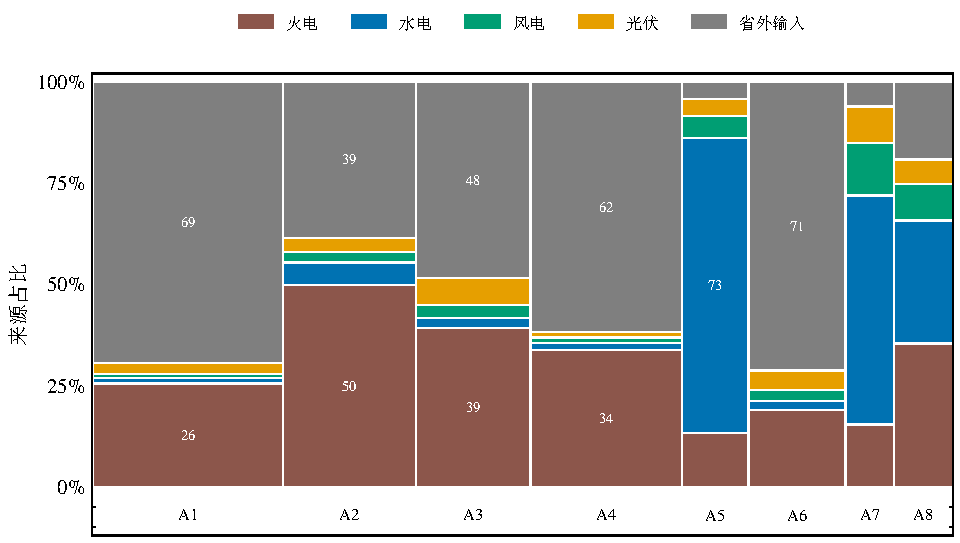
\includegraphics[width=0.88\textwidth]{../src/outputs/q2/fig_q2_origin_mix.pdf}
\caption{各区域终端用电来源的马赛克图。列宽正比于 2025 年用电量，块高为来源份额；A5/A7 以水电为主，A1/A4/A6 以省外输入为主。}
\label{fig:originmix}
\end{figure}

图\ref{fig:q2season}把同一分解拆到月份：A5/A7 的水电份额在 4至8 月抬升，火电与输入被挤出，与碳势夏季低谷同相；A2/A4 各月火电加输入始终占主导，所以碳势全年高位。图\ref{fig:q2sankey}用冲积图汇总来源到消费区的能量去向：省外输入主要进入 A1/A4/A6，水电集中供给 A5/A7。

\begin{figure}[H]
\centering
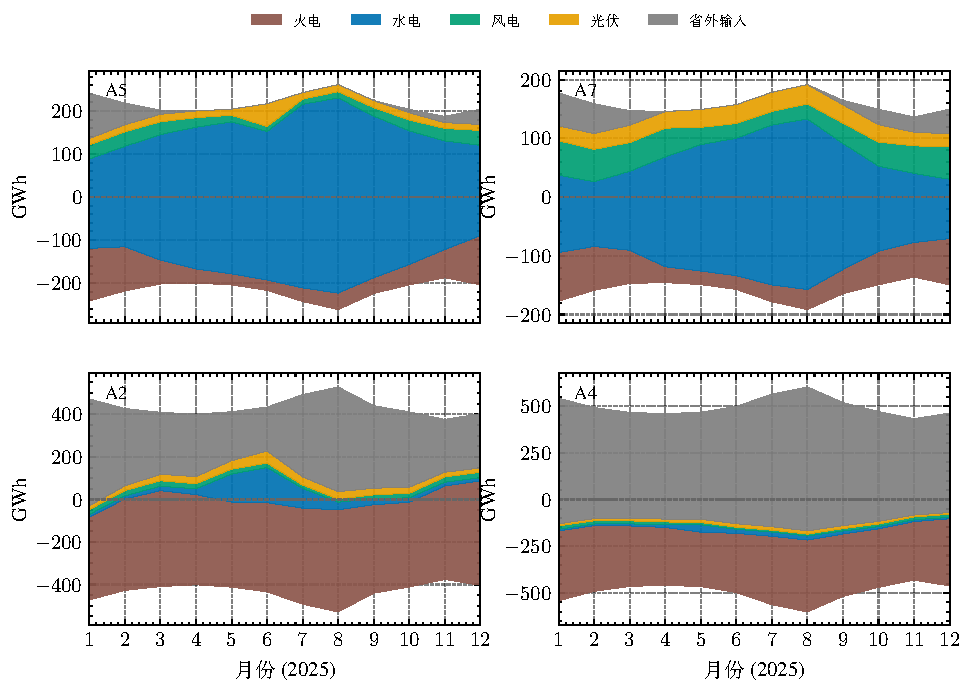
\includegraphics[width=0.92\textwidth]{../src/outputs/q2/fig_q2_seasonal_mix.pdf}
\caption{典型区域逐月电源结构对称流图。带宽正比于终端电量、中线为零；A5/A7 丰水期水电带变宽，A2 火电、A4 省外输入全年占优。}
\label{fig:q2season}
\end{figure}

\begin{figure}[H]
\centering
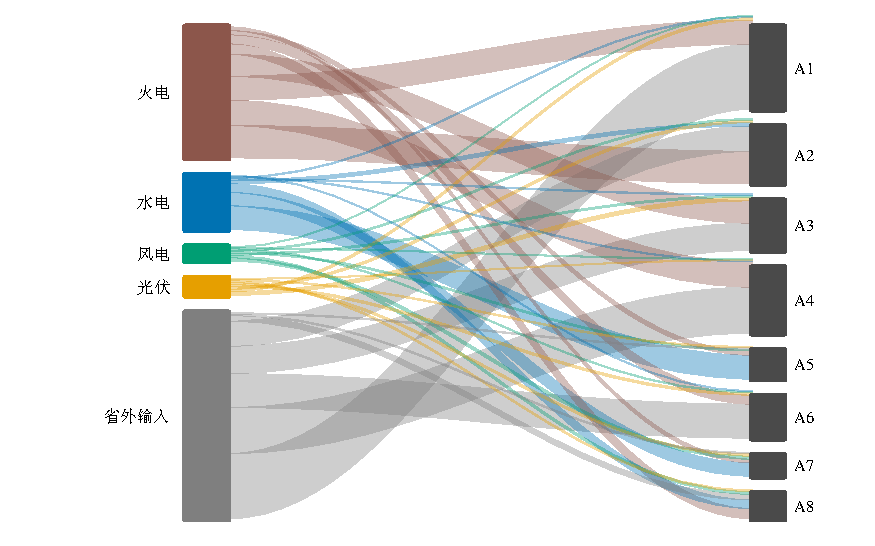
\includegraphics[width=0.92\textwidth]{../src/outputs/q2/fig_q2_sankey.pdf}
\caption{2025 年电源来源$\to$消费区能量冲积图。带宽度正比于电量；省外输入流向 A1/A4/A6，水电流向 A5/A7。}
\label{fig:q2sankey}
\end{figure}

\begin{figure}[H]
\centering
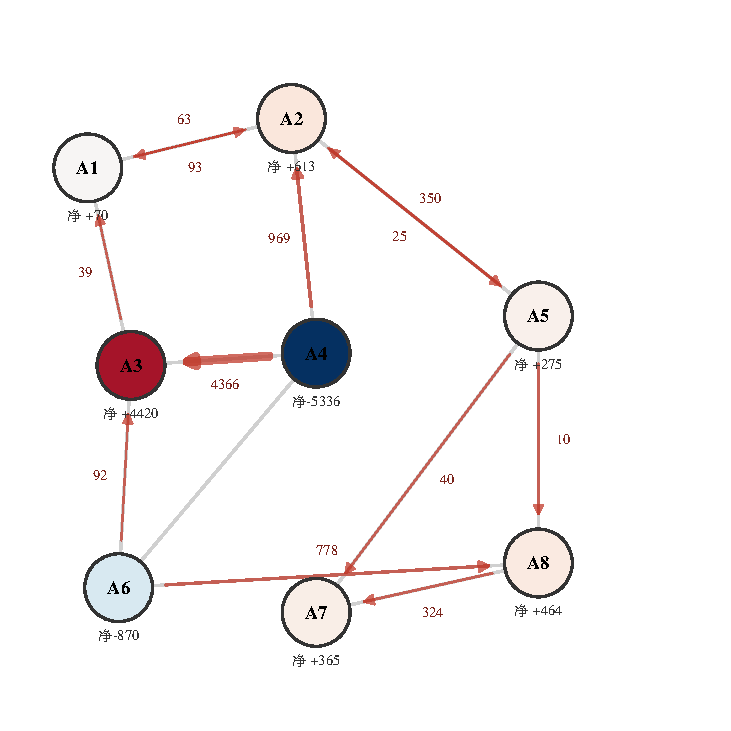
\includegraphics[width=0.88\textwidth]{../src/outputs/deepen/fig_q2_carbon_flow_network.pdf}
\caption{2025 年区域间电力碳流与净责任格局。箭头宽度正比于到达碳量 $F_{j\to i}$（ktCO$_2$）；节点颜色为 $C^+_i-P^+_i$（红=净转入）。主路径为 A4$\to$A3（4366.34\,kt）。}
\label{fig:cfnet}
\end{figure}

\begin{figure}[H]
\centering
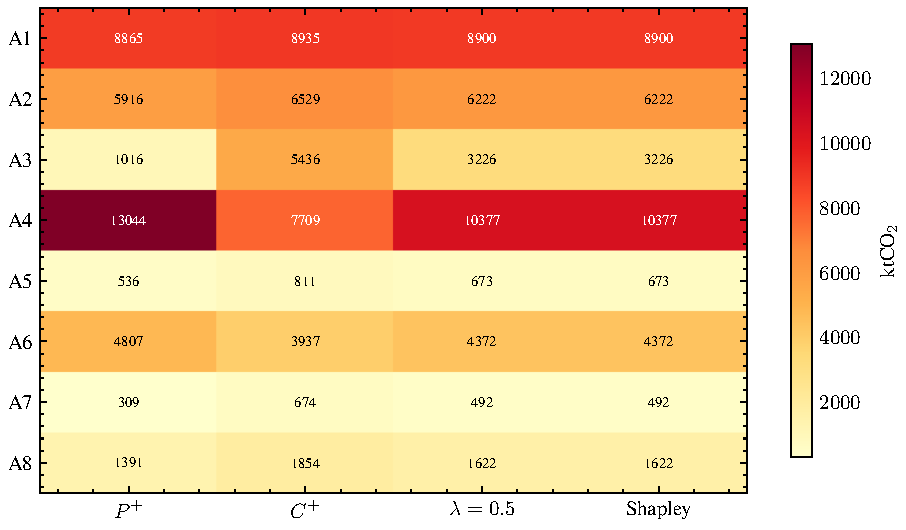
\includegraphics[width=0.92\textwidth]{../src/outputs/deepen/fig_q2_responsibility_shapley.pdf}
\caption{四种口径下的区域碳排放责任热力图（2025）。$\lambda=0.5$ 与 Shapley 两列数值重合，源于式\eqref{eq:shapley}的结构恒等式；A4 为净转出、A3 为净转入。}
\label{fig:resp}
\end{figure}

\begin{table}[htbp]
\centering
\caption{2025 年区域碳排放责任与 Shapley 共担（ktCO$_2$）}
\label{tab:resp}
\resizebox{\textwidth}{!}{
\begin{tabular}{lrrrrr}
\toprule
区域 & $P^+$ & $C^+$ & $\lambda=0.3$ & $\lambda=0.5$ & Shapley \\
\midrule
A1 & 8865.08 & 8934.69 & 8913.81 & 8899.88 & 8899.89 \\
A2 & 5915.76 & 6528.65 & 6344.78 & 6222.20 & 6222.21 \\
A3 & 1015.92 & 5435.60 & 4109.70 & 3225.76 & 3225.76 \\
A4 & 13044.48 & 7708.95 & 9309.61 & 10376.72 & 10376.72 \\
A5 & 535.50 & 810.80 & 728.21 & 673.15 & 673.15 \\
A6 & 4807.07 & 3936.72 & 4197.82 & 4371.89 & 4371.89 \\
A7 & 309.30 & 674.02 & 564.60 & 491.66 & 491.66 \\
A8 & 1390.66 & 1854.35 & 1715.24 & 1622.50 & 1622.50 \\
合计 & 35883.77 & 35883.78 & 不适用 & 不适用 & 35883.78 \\
\bottomrule
\end{tabular}}
\end{table}

\subsection{条件参数自举与下游触限风险}

附件未提供跨年度重复的 2025 量测，因此无法识别无条件真实分布。本文采用 500 次条件参数自举\cite{Sun2024probabilistic}：以问题一拟合状态为条件真值，按照各量测类型的 $\sigma$ 独立生成截断于零的正态伪观测，并保留原缺失模式与结构性零流量；每个样本均从伪观测出发重新完成 Huber 调和，再求解 12 个 $8\times8$ 碳势系统。随机种子固定为 20250822。2025 年排放因子、网络、工程先验和量测精度保持不变，附件 6 给出的未来因子区间不作为 2025 年的概率分布。

500/500 个样本成功。最大能量平衡残差为 $1.01\times10^{-12}$\,GWh，碳流系统最大条件数为 6.606，责任守恒最大相对误差为 $4.03\times10^{-16}$，最终分位端点的最大 Monte Carlo 标准误为 0.0001198\,kgCO$_2$/kWh。图\ref{fig:q2uncertainty}显示 A4、A5 的年均强度点估计及 95\% 条件区间分别为 $0.62399\,[0.62179,0.62537]$ 和 $0.15217\,[0.15019,0.15320]$；500 次中 A4 始终最高、A5 始终最低，相应概率的 Wilson 95\% 下界均为 0.9924。

\begin{figure}[H]
\centering
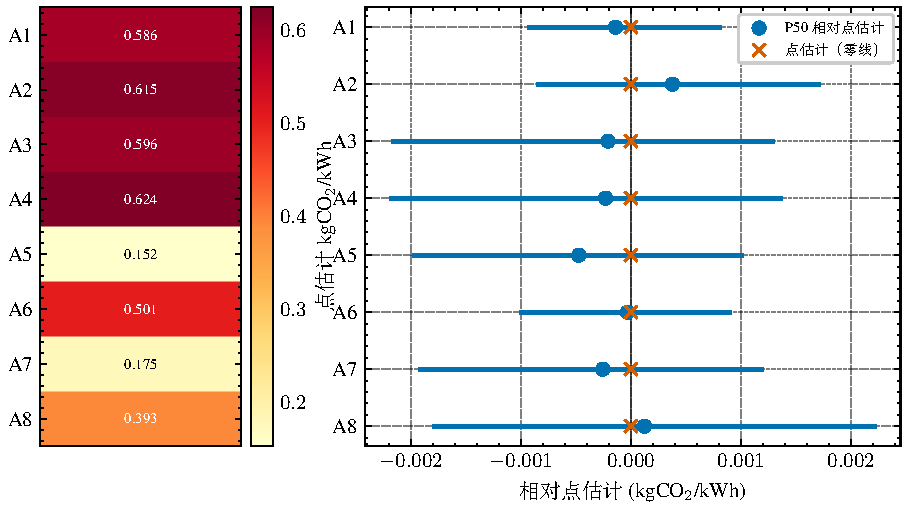
\includegraphics[width=0.90\textwidth]{../src/outputs/q2/fig_q2_uncertainty.pdf}
\caption{八区域年均终端碳强度：左侧色带为调和后点估计，右侧把 95\% 条件区间画成相对点估计的偏差（圆点为 P50）。区间宽度约 $0.002$至$0.004$，在原强度轴上会被点标盖住。}
\label{fig:q2uncertainty}
\end{figure}

A4$\to$A3 年度到达碳流的条件 P2.5/P50/P97.5 为 4356.76/4387.27/4419.04\,kt，见图\ref{fig:q2channeluncertainty}。将同一批样本传递至问题三固定的 $\varepsilon=1\%$ 推荐计划，且不针对单个样本重新优化，得到 2026至2030 年省级触限概率依次为 0、0.2\%、32.0\%、35.8\%、35.8\%。尽管点估计未超过上限，后三年的触限概率仍高于 30\%，实际执行时需要设置动态重估触发条件。这些区间未覆盖排放因子、未来结构、相关量测误差和模型错设，因而不属于无条件预测区间。

\begin{figure}[H]
\centering
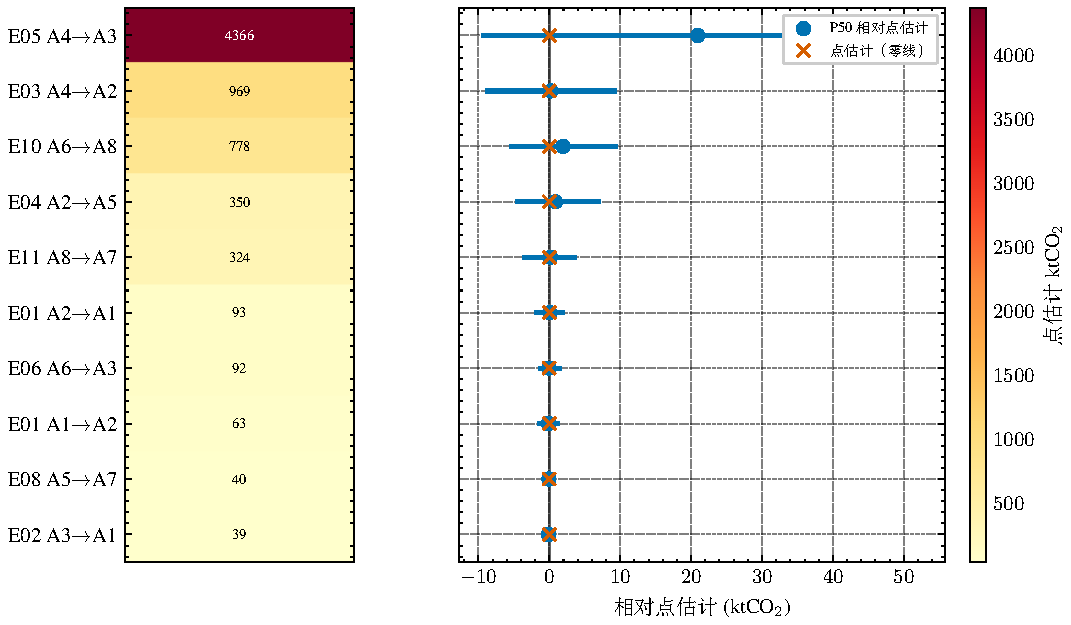
\includegraphics[width=0.92\textwidth]{../src/outputs/q2/fig_q2_channel_carbon_uncertainty.pdf}
\caption{前十条通道的年度到达碳流。左侧色带为点估计（以 A4$\to$A3 为主），右侧为相对点估计的 95\% 条件区间。各通道量级相差两个数量级，右图采用偏差轴以同时显示各区间。}
\label{fig:q2channeluncertainty}
\end{figure}

\section{问题三：区域碳预算与五年项目组合}

\subsection{预算分解}

全省消费侧年度上限 $\overline E_y$ 为硬约束。区域软预算采用惯性份额与公平份额的凸组合\cite{Raupach2014sharing,Zhou2016carbon,Wang2013regional}
\begin{equation}
B_{i,y}=\bigl[w_y\pi_i+(1-w_y)d_{i,y}\bigr]\overline E_y,
\label{eq:budget}
\end{equation}
其中 $\pi_i$ 为 2025 年 $C^+$ 份额，$d_{i,y}$ 为当年需求份额，$w_y$ 由 2026 年的 0.85 线性降到 2030 年的 0.65。超额 $b_{i,y}=\max(0,E_{i,y}-B_{i,y})$ 按 0.2 百万元/kt（约 200 元/tCO$_2$）计罚。

\subsection{投资与运行耦合 MILP}

决策变量为项目 $p$ 在年份 $t$ 的开工规模 $x_{p,t}$（通道升级为 0-1）。运行层包含本地电源上限、省外输入年容量、通道容量与问题一校正后的 $\eta_e$，以及最低供能率。碳核算按附件 4B 的官方简化式
\begin{equation}
E_{i,y}=\rho_i\kappa_y(D_{i,y}-G^{\mathrm{PV}}_{i,y})+0.045\,G^{\mathrm{PV}}_{i,y}-A_{i,y},
\label{eq:E}
\end{equation}
交通电气化新增用电计入 $D$，燃油替代计入直接减排 $A$，不重复计算。$\rho_i$ 取问题二 2025 年终端碳强度。总规模、年开工上限、五类施工资源、年度投资上限、互斥与协同触发均作为硬约束，协同项用 McCormick 线性化。保留下式作为传统加权罚比较基线：
\begin{equation}
\min J_w=\sum_{p,t}\frac{c_p x_{p,t}}{(1+r)^{t-2026}}
+0.2\sum_{i,y}b_{i,y}
+10\sum_{i,y}(D_{i,y}-s_{i,y}),
\label{eq:obj}
\end{equation}
其中 $b_{i,y}=\max(0,E_{i,y}-B_{i,y})$，主口径 $r=0$。式\eqref{eq:obj}中的系数 0.2 人为规定了公平与成本之间的交换率，因此该目标仅作为比较基线。正式方案采用严格词典序 $\varepsilon$-约束：先最小化总缺供 $S$，再在 $S=S^*$ 下最小化投资 $C$，最后在 $C\le(1+\varepsilon)C^*$ 内最小化最大相对区域超额 $R$，并以投资最小打破同值解：
\begin{equation}
\begin{aligned}
S^*&=\min S(x),\\
C^*&=\min\{C(x):S(x)\le S^*\},\\
R^*(\varepsilon)&=\min\bigl\{R:\ C(x)\le(1+\varepsilon)C^*,
b_{i,y}(x)\le R B_{i,y},\ \forall i,y\bigr\}.
\end{aligned}
\label{eq:epsilon}
\end{equation}
该结构仍是多年期投资与运行耦合 MILP\cite{Koltsaklis2018generation}。各阶段均由 HiGHS 精确求解并独立回代，避免直接加总不同量纲的目标。

\subsection{\texorpdfstring{词典序 $\varepsilon$-Pareto 结果}{词典序 ε-Pareto 结果}}

阶段一得到 $S^*=0$，阶段二得到最低投资 $C^*=964.9697$ 百万元。扫描 $\varepsilon\in\{0,0.5\%,1\%,2\%,5\%\}$ 的结果见表\ref{tab:epsilon}与图\ref{fig:epsilon}。随着投资容许度扩大，最大相对区域超额单调下降。该曲线明确给出成本与区域负担之间的交换关系，而单一罚系数无法呈现这一关系。

\begin{table}[htbp]
\centering
\caption{零缺供条件下投资与最大相对区域超额的 $\varepsilon$-Pareto 前沿}
\label{tab:epsilon}
\begin{tabular}{ccccc}
\toprule
$\varepsilon$ & 实际投资（百万元） & 相对 $C^*$ 增投 & 最大相对超额 & 项目数 \\
\midrule
0 & 964.970 & 0.000\% & 8.377\% & 6 \\
0.5\% & 969.783 & 0.499\% & 7.964\% & 7 \\
1\% & 974.603 & 0.998\% & 7.611\% & 6 \\
2\% & 984.247 & 1.998\% & 7.100\% & 7 \\
5\% & 1013.040 & 4.982\% & 6.707\% & 8 \\
\bottomrule
\end{tabular}
\end{table}

\begin{figure}[H]
\centering
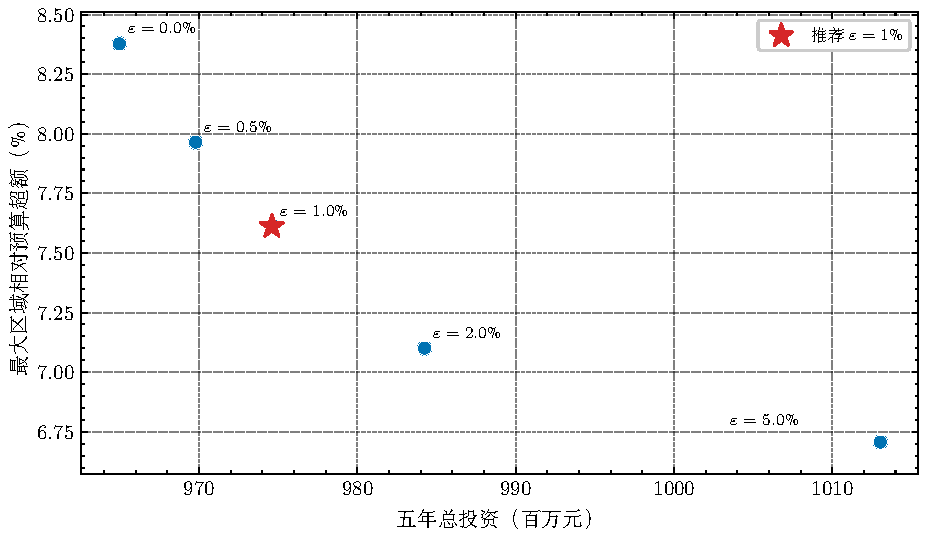
\includegraphics[width=0.90\textwidth]{../src/outputs/q3/fig_q3_epsilon_pareto.pdf}
\caption{$\varepsilon$-Pareto 前沿散点：横轴为五年投资，纵轴为最大区域相对预算超额。星号为推荐点 $\varepsilon=1\%$。}
\label{fig:epsilon}
\end{figure}

推荐 $\varepsilon=1\%$：实际投资 974.6028 百万元，较 $C^*$ 增加 0.9983\%，最大相对超额为 7.6112\%。加权基线投资 973.9 百万元、最大相对超额 8.2808\%，推荐方案的投资仅增加约 0.70 百万元。区域超额总量由 4575.58 增至 4631.89\,kt，原因是优化目标控制最坏相对负担，而非超额总和。推荐方案包含 P12、P15、P16、P19、P23、P31 六个项目，2026至2030 年投资分别为 543.35、270.13、83.30、77.82、0 百万元，碳裕度为 327.2、58.2、3.1、0、0\,kt。最大独立约束回代误差为 $2.05\times10^{-12}$，五个 Pareto 点均达到最优，MILP gap 为 0。

无项目五年累计越限 560.4\,kt；按单位减排成本补到上限的贪心解投资 965.0 百万元。表\ref{tab:base}把这些可解释基线与两个 MILP 方案并列。2030 年碳上限的有限差分影子价格为 3.1616 百万元/kt，它只表示一次性投资目标下的局部规划边际成本，不宜直接当作市场碳价。问题二的量测自举还给出：固定推荐计划在 2028至2030 年的条件触限概率为 32.0\%、35.8\%、35.8\%，实际执行需要留动态安全裕度。

\begin{figure}[H]
\centering
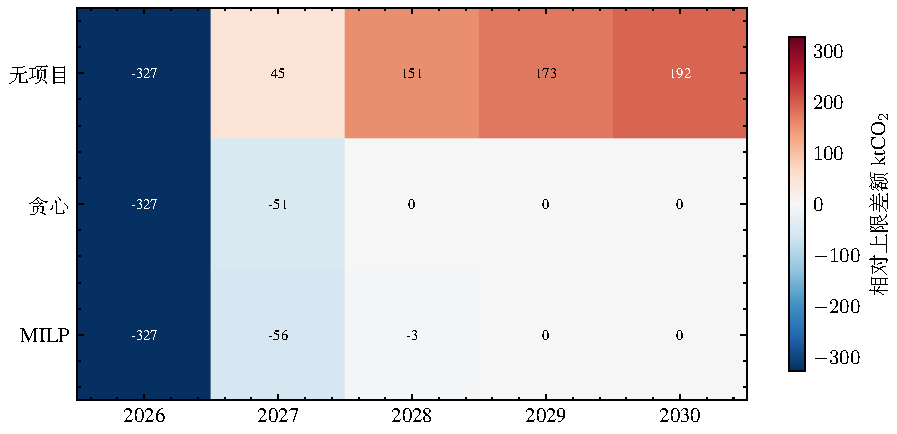
\includegraphics[width=0.92\textwidth]{../src/outputs/deepen/fig_q3_no_project.pdf}
\caption{无项目、贪心与 MILP 相对碳上限的差额热力图。正值越限、负值裕度；最终推荐由图\ref{fig:epsilon}的词典序前沿给出。}
\label{fig:noproj}
\end{figure}

\begin{table}[htbp]
\centering
\caption{无项目、贪心与两类 MILP 方案比较}
\label{tab:base}
\begin{tabular}{lccccc}
\toprule
方案 & 投资 & 五年总越限 & 区域超额合计 & 最大相对超额 & 项目数 \\
\midrule
无项目 & 0 & 560.4 & 5078.7 & 不适用 & 0 \\
贪心（补到上限） & 965.0 & 0 & 4642.2 & 不适用 & 6 \\
加权罚基线 & 973.9 & 0 & 4575.58 & 8.281\% & 7 \\
$\varepsilon=1\%$ 推荐 & 974.603 & 0 & 4631.89 & 7.611\% & 6 \\
\bottomrule
\end{tabular}
\end{table}

\section{问题四：送端碳不确定与鲁棒滚动}

\subsection{冲击如何传到消费侧}

为保持比较口径一致，问题四的压力测试沿用问题三的加权罚基线（投资 973.9 百万元）；$\varepsilon=1\%$ 推荐计划的量测触限风险已在问题二列出。加权基线在 2028至2030 年接近省级上限，送端碳因子上升时几乎没有剩余裕度。记 $\xi_{j,y}$ 为接入区 $j$ 的因子乘数。若将进口偏差直接计入接入区碳账，会与 $\rho\kappa$ 基线重复计算。与问题二一致的传导方式是先根据 2025 年份额计算“源自 $j$ 的消费电量” $W_{j,y}=\sum_i(D_{i,y}-G^{\mathrm{PV}}_{i,y})S_{ij}$，再令
\begin{equation}
\Delta E_y=\kappa_y\sum_j \bar e_j(\xi_{j,y}-1)W_{j,y}.
\label{eq:dE}
\end{equation}
将 $S_{ij}$ 固定在 2025 年水平是一项较强假设。若只计接入区进口电量而忽略转供，S3-2030 增量由 454.5 降至 437.8\,kt（$-3.7\%$）；若再将 $S$ 向 A4 集中 20\%，增量则升至 495.7\,kt。当前模型只描述给定来源份额下的因子冲击，未覆盖 $S$ 的长期漂移。

\subsection{\texorpdfstring{压力测试与双口径 POR}{压力测试与双口径 POR}}

加权基线在 S3 的 2028/2029/2030 年越限为 195.6/338.5/454.5\,kt；完整 $\Gamma$ 集的逐年最坏越限为 244.4/394.2/486.9\,kt，合计 1125.49\,kt。对 $\xi$ 采用预算不确定集\cite{Bertsimas2004price}
\begin{equation}
\mathcal U_y(\Gamma_y)=\bigl\{\boldsymbol z:\ 0\le z_j\le 1,
\textstyle\sum_j z_j\le \Gamma_y\bigr\},
\label{eq:budgetset}
\end{equation}
内层最大增量对偶化为 $\Gamma_y\pi_y+\sum_j\mu_{j,y}$ 后代入 MILP。当前 POR 模型允许省级碳缺口，并按 50 百万元/kt 处罚，因此得到的是软风险方案；求解器返回可行不代表硬约束下可行。扫描 $\tau\Gamma$ 后，需要分别报告设计集 $\mathcal U(\tau\Gamma)$ 上的违约，以及将全部方案置于统一 $\mathcal U(\Gamma)$ 下得到的回测违约，见表\ref{tab:gamma}。

\begin{table}[htbp]
\centering
\caption{$\Gamma$ 缩放下的双口径 price of robustness}
\label{tab:gamma}
\begin{tabular}{cccc}
\toprule
$\tau$ & 投资（百万元） & 设计集 $\tau\Gamma$ 违约 & 统一 $\Gamma$ 回测违约 \\
\midrule
0.0 & 973.9 & 0.00 & 1125.49 \\
0.5 & 3375.5 & 0.00 & 338.15 \\
1.0 & 4834.5 & 14.85 & 14.85 \\
1.5 & 5160.4 & 166.63 & 14.89 \\
2.0 & 5160.4 & 211.34 & 14.89 \\
\bottomrule
\end{tabular}
\end{table}

$\tau>1$ 时设计集扩大，而项目与资源上限不变，因而软违约上升；统一 $\Gamma$ 回测下的违约并未随之增加。$\tau=1$ 的软方案投资 4834.5 百万元，较确定性基线增加 3860.6 百万元，但仍存在 14.85\,kt 缺口。

\begin{figure}[H]
\centering
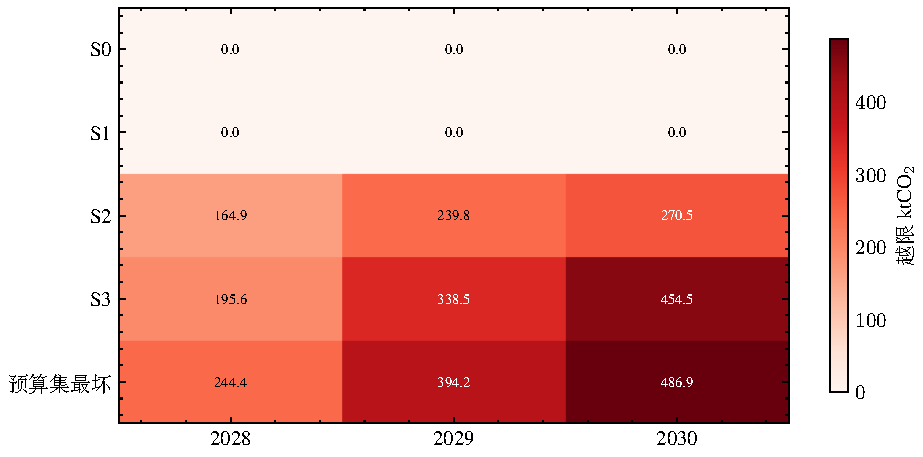
\includegraphics[width=0.92\textwidth]{../src/outputs/q4/fig_q4_stress.pdf}
\caption{问题三加权罚基线的越限热力图（情景$\times$年份）。S0 全零，S3-2030 为 454.5\,kt。}
\label{fig:stress}
\end{figure}

\begin{figure}[H]
\centering
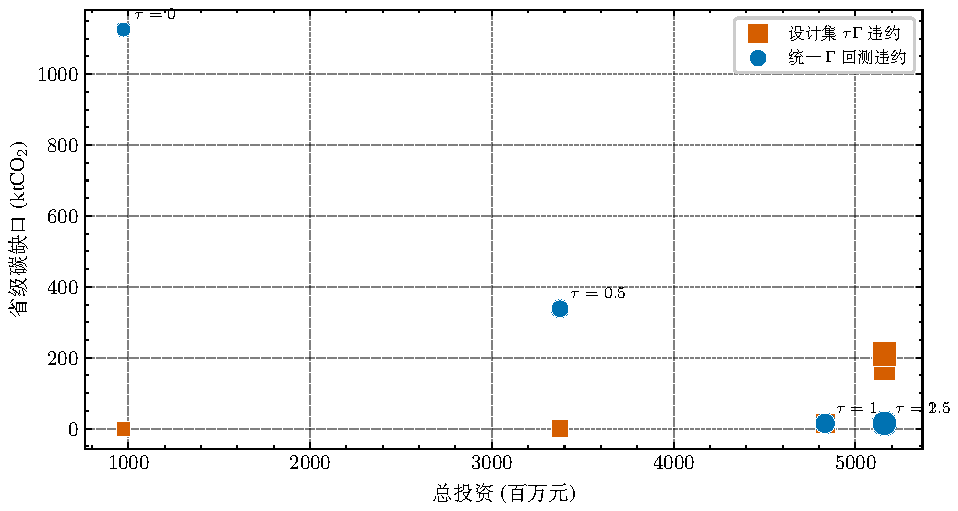
\includegraphics[width=0.92\textwidth]{../src/outputs/q4/fig_q4_por.pdf}
\caption{鲁棒性代价的气泡散点。横轴投资、纵轴碳缺口，气泡大小随 $\tau$ 增大；圆点为统一 $\Gamma$ 回测，方点为设计集违约。}
\label{fig:por}
\end{figure}

\subsection{硬可行半径与恢复边界}

去掉碳缺口松弛后，完整硬可行半径定义为
\begin{equation}
\tau^*=\max\bigl\{\tau:\ \exists x,\ E_y(x,\xi)\le\bar E_y,
\ \forall\xi\in\mathcal U_y(\tau\Gamma_y),\ \forall y\bigr\}.
\label{eq:taustar}
\end{equation}
二分求得 $\tau^*=0.95300293$，对应投资 4724.64 百万元。在题设投资和资源上限下，完整 $\Gamma=1$ 没有硬零越限方案。若按“先最小总缺口、再最小投资”求解，$\Gamma=1$ 的不可避免总缺口为 14.848813\,kt，其中 2028 年 6.151329、2029 年 8.697484\,kt，其余年份为 0。

硬可行性可通过单独放宽一种约束恢复。二分得到的临界包络为
\begin{equation}
f_{\rm inv}\in(1.0553207,1.0553284],\qquad
f_{\rm res}\in(1.0449982,1.0450058],
\label{eq:restore}
\end{equation}
即年度投资上限按保守上界需放宽 5.5328\%，或将五类施工资源统一放宽 4.5006\%。两个上界均经独立完整 $\Gamma$ 回测确认零越限，各自略低的下界则由求解器证明不可行。若不放宽长期施工约束，则需另行引入绿电购买、需求响应或碳抵消。由于题面未给出这些资源的价格，本文不额外假设其单点成本。

本文还采用“先求当前场景，再加入所发现的最坏场景后重解”的方式构造软防御，得到两个场景，目标值为 6344.7 百万元。该过程未求解标准两阶段 ARO 的分离子问题，也未维护上下界与收敛 gap。按照严格 C\&CG 的定义\cite{Zeng2013solving}，该方法属于可行性场景生成启发式，不能保证得到全局最优的可调鲁棒解。

\subsection{四路径非预见最小最大相对遗憾}

S0至S3 是无概率典型路径，不能设等概率求期望。令 $C_s^*$ 为路径 $s$ 的完美信息（PI）硬碳上限最优目标；令 2026至2027 开工 $x^0$ 对四路径共享，2028至2030 在年初识别路径后用 $x^s$ 追索。采用混合整数追索的最小最大相对遗憾思想\cite{BenTal2004adjustable,Barkom2025regret}：
\begin{equation}
\min R,\qquad
\frac{C_s(x^0,x^s)-C_s^*}{C_s^*}\le R,
\quad s\in\{S0,S1,S2,S3\},
\label{eq:regret}
\end{equation}
并对四条路径分别施加硬碳上限。模型包含 2471 个变量、146 个二元变量和 3389 条约束，可由 HiGHS 直接求解。

\begin{table}[htbp]
\centering
\caption{四条典型路径的完美信息基准与非预见最小最大遗憾解}
\label{tab:regret}
\begin{tabular}{lrrrr}
\toprule
路径 & PI 目标 & 非预见目标 & 非预见投资 & 相对遗憾 \\
\midrule
S0 & 1912.873 & 2933.102 & 2094.466 & 53.335\% \\
S1 & 1214.056 & 2933.102 & 2094.466 & 141.595\% \\
S2 & 3782.083 & 3820.201 & 3020.995 & 1.008\% \\
S3 & 5239.442 & 5258.148 & 4490.793 & 0.357\% \\
\bottomrule
\end{tabular}
\end{table}

\begin{figure}[H]
\centering
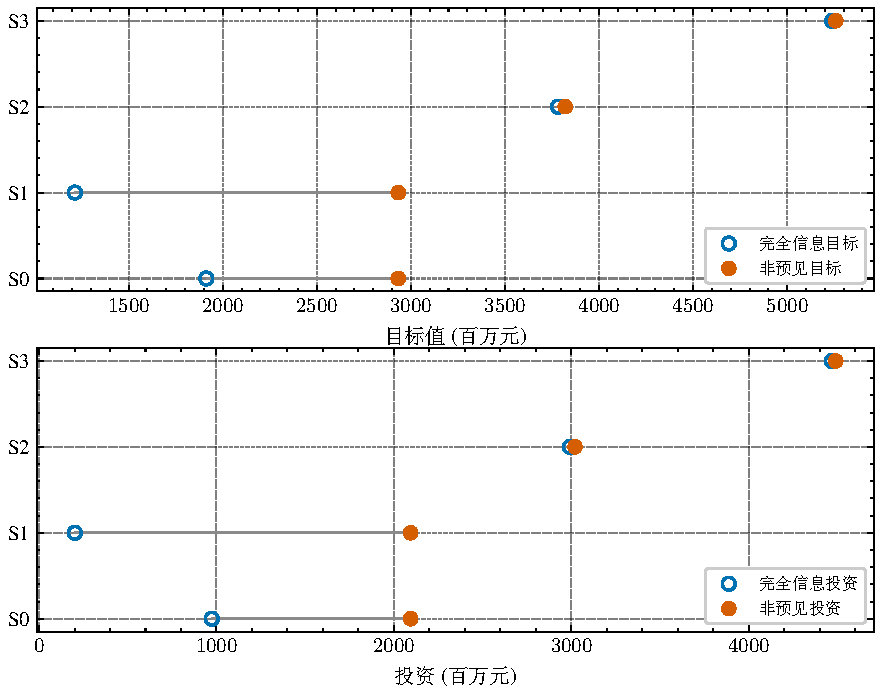
\includegraphics[width=0.92\textwidth]{../src/outputs/q4/fig_q4_regret.pdf}
\caption{四路径完美信息与非预见方案的哑铃图。茎长即绝对遗憾；S1 的 PI 基数最小，早期共同防御使其相对遗憾最高。}
\label{fig:regret}
\end{figure}

共享一阶段投资为 2094.466 百万元，四条路径均实现硬零越限。S1 的 PI 目标最小，因此相对遗憾最高。表\ref{tab:regret}同时列出绝对目标，以避免仅依据百分比作出偏差判断。

\subsection{滚动 objective-to-go 的比较口径}

沿 S3 路径，在每年年初用已观测因子重解、对未观测年份保留 $\Gamma$ 软防御\cite{Silvente2015rolling}。信息比较固定同一决策时点与同一已承诺状态，只比较“使用/不使用本年观测”的剩余期目标，结果见表\ref{tab:rolling}。

\begin{table}[htbp]
\centering
\caption{S3 滚动中同状态 objective-to-go 的信息改善（百万元）}
\label{tab:rolling}
\begin{tabular}{lrrr}
\toprule
决策年 & 使用本年观测 & 不使用本年观测 & 目标改善 \\
\midrule
2028 & 3307.766 & 3615.333 & 307.566 \\
2029 & 1445.621 & 1880.495 & 434.874 \\
2030 & 191.775 & 191.775 & 0 \\
\bottomrule
\end{tabular}
\end{table}

目标改善中包含避免的软违约罚，因此不能将 307.566 或 434.874 百万元解释为等额投资节省；跨年份比较包含沉没成本的全周期目标也不具可比性。S3 滚动最终投资仍为 4834.5 百万元，并在该路径上实现零越限，但这不构成对完整 $\Gamma$ 集的硬保证。滚动模型保留了观测后的追索接口。完整压力下的底线仍由 $\tau^*$、14.8488\,kt 最小缺口和上述资源恢复边界共同确定。

\section{问题五：决策咨询报告}

{\heiti 关于“十五五”电力低碳转型的决策建议}

{\kaishu （呈省级能源主管部门）}

\vspace{0.3em}
对 2025 年多源监测数据的守恒校验得到 23 项诊断标记，包括月度与年度系统最大 8.7\% 的口径差、E10 年度“受端大于送端”、E03 单月隐含线损 17.5\% 以及 4 处缺失。采用单次凸 Huber 调和后，最大能量平衡残差为 $4.89\times10^{-13}$\,GWh；E05 年度线损为 0.01675（工程值 0.020），E07 因全年无有效流量只能保留工程值 0.027。最值得复核的依次是 E10 年度送、受端汇总和 A4 八月省外输入。建议把关口月表与年度汇总统一编码，并对 E10 设置自动对账告警。

A4、A5 年均终端碳强度分别为 0.62399 和 0.15217\,kgCO$_2$/kWh。A3 消费责任为 5435.60\,kt，是扩展生产责任的 5.35 倍，主碳流 A4$\to$A3 为 4366.34\,kt。500 次完整量测自举给出该主碳流 95\% 条件区间 $[4356.76,4419.04]$\,kt，所有样本均保持 A4 最高、A5 最低的排序。区域考核宜同时公开生产侧与消费侧两套口径。五五共担可作为协商起点，但其与当前 Shapley 值一致是结构恒等式，数据并未给出唯一的公平权重。

项目方案根据 $\varepsilon$-前沿选择。零缺供最低投资为 964.970 百万元；推荐 $\varepsilon=1\%$，投资 974.603 百万元，较最低投资增加 0.998\%，加权基线的最大区域相对超额则从 8.281\% 降至 7.611\%。六个入选项目为 P12、P15、P16、P19、P23、P31，主要投向分布式光伏和交通电气化。2030 年有限差分影子价格 3.1616 百万元/kt 只是当前项目库和一次性投资口径下的局部规划信号，不宜直接作为市场碳价。量测误差传播显示，固定推荐计划在 2028至2030 年的条件触限概率分别为 32.0\%、35.8\%、35.8\%。尽管点估计仍在上限以内，2028 年后的触限概率已超过 30\%，因此需要按年重估。

若省外来电沿高碳路径 S3 变化，加权基线到 2030 年将超出上限 454.5\,kt。完整 $\Gamma=1$ 在现有投资和施工资源上限下不存在硬零越限方案。软防御投资达到 4834.5 百万元后，仍有 14.8488\,kt 的最小缺口，硬可行半径为 $\tau^*=0.953003$。若监管要求覆盖完整 $\Gamma$，可将年度投资上限至少放宽至 1.0553284 倍，或将五类施工资源统一放宽至 1.0450058 倍。若两类约束均不放宽，则需配置绿电购买、需求响应等应急资源，并纳入真实报价后重新优化。

执行阶段应先依据完整 $\Gamma$ 的恢复边界配置资源。S0至S3 的非预见方案用于安排 2026 年和 2027 年开工项目，此后按年滚动。四路径最小最大遗憾方案的前两年共享投资为 2094.466 百万元，四条路径均满足硬约束。最大相对遗憾 141.595\% 来自低成本 S1 路径上的早期防御机会成本。S3 滚动使 2028、2029 年同状态剩余期目标分别改善 307.566、434.874 百万元，其中包含避免的违约罚，不能解释为等额投资节省。建议每年三季度更新送端因子区间和来源份额，次年年初根据已确认状态调整未开工项目，并以完整 $\Gamma$ 恢复边界复核应急资源是否充足。

\section{模型评价、局限性与结论}

各环节均进行了独立回代与对照检验。问题一比较了 Huber 与 WLS 在污染数据下的表现；问题二的 500 个自举样本均重新执行上游调和；问题三的五个 $\varepsilon$ 点均单独校验约束。问题四分别报告设计集与统一集、软约束与硬约束、完美信息目标与非预见目标，避免混用评价口径。

问题二给出的区间以独立正态量测误差、固定排放因子和固定网络为条件，未包含相关误差、模型错设和未来结构，因此不构成无条件置信保证。$S_{ij}$ 被固定至 2030 年，而忽略转供以及将份额向 A4 集中 20\% 的敏感性结果表明，枢纽份额漂移仍需按年重算。题面官方规划式采用平均碳强度，而非边际排放，且未提供电抗、机组成本和启停参数，因此本模型不属于 Carbon-Aware OPF，通道升级的碳价值也可能被低估。$\lambda=0.5$ 与 Shapley 一致源于特征函数结构，无法回答政策公平权重是否唯一。S0至S3 没有给定概率，最小最大遗憾结果会受到典型路径集合的影响；完整 $\Gamma$ 也只是压力集合，并非概率分布。题面还缺少应急资源和碳抵消价格，本文仅给出恢复硬可行性所需的资源边界，不估计最优采购成本。

电量经稳健守恒调和后进入碳流核算，碳责任结果同时报告条件区间。五五共担可作为协商起点，但不是唯一公平解。基准规划推荐投资 974.603 百万元的 $\varepsilon=1\%$ 方案，并根据量测触限概率预留动态裕度。现有资源无法覆盖完整送端压力，执行时应以 $\tau^*$ 和恢复边界为约束底线，再结合非预见路径方案逐年更新剩余期目标。

\begin{sloppypar}
\begin{thebibliography}{99}
\bibitem{Crowe1996data} Crowe C M. Data reconciliation: Progress and challenges[J]. Journal of Process Control, 1996, 6(2-3): 89-98.
\bibitem{Narasimhan1999data} Narasimhan S, Jordache C. The Importance of Data Reconciliation and Gross Error Detection[M]//Data Reconciliation and Gross Error Detection. Elsevier, 1999: 1-31.
\bibitem{Schweppe1970power} Schweppe F C, Wildes J. Power System Static-State Estimation, Part I: Exact Model[J]. IEEE Transactions on Power Apparatus and Systems, 1970, PAS-89(1): 120-125.
\bibitem{Abur2004power} Abur A, Expósito A G. Power System State Estimation: Theory and Implementation[M]. CRC Press, 2004.
\bibitem{deChalendar2021physics} de Chalendar J A, Benson S M. A physics-informed data reconciliation framework for real-time electricity and emissions tracking[J]. Applied Energy, 2021, 304: 117761.
\bibitem{Liu2023robust} Liu Z, Li P, Wang C, et al. Robust State Estimation of Active Distribution Networks with Multi-source Measurements[J]. Journal of Modern Power Systems and Clean Energy, 2023, 11(4): 1540-1552. DOI: 10.35833/MPCE.2022.000200.
\bibitem{Bialek1996tracing} Bialek J. Tracing the flow of electricity[J]. IEE Proceedings - Generation, Transmission and Distribution, 1996, 143(4): 313.
\bibitem{Kang2015carbon} Kang C, Zhou T, Chen Q, et al. Carbon Emission Flow From Generation to Demand: A Network-Based Model[J]. IEEE Transactions on Smart Grid, 2015, 6(5): 2386-2394.
\bibitem{Sun2024probabilistic} Sun X, Bao M, Ding Y, et al. Modeling and evaluation of probabilistic carbon emission flow for power systems considering load and renewable energy uncertainties[J]. Energy, 2024, 296: 130768. DOI: 10.1016/j.energy.2024.130768.
\bibitem{Peters2008production} Peters G P. From production-based to consumption-based national emission inventories[J]. Ecological Economics, 2008, 65(1): 13-23.
\bibitem{Davis2010consumption} Davis S J, Caldeira K. Consumption-based accounting of CO$_2$ emissions[J]. Proceedings of the National Academy of Sciences, 2010, 107(12): 5687-5692.
\bibitem{Gallego2005consistent} Gallego B, Lenzen M. A consistent input-output formulation of shared producer and consumer responsibility[J]. Economic Systems Research, 2005, 17(4): 365-391.
\bibitem{Lenzen2007shared} Lenzen M, Murray J, Sack F, et al. Shared producer and consumer responsibility: Theory and practice[J]. Ecological Economics, 2007, 61(1): 27-42.
\bibitem{Qin2020cooperative} Qin Q, Liu Y, Huang J P. A cooperative game analysis for the allocation of carbon emissions reduction responsibility in China's power industry[J]. Energy Economics, 2020, 92: 104960.
\bibitem{Feng2013outsourcing} Feng K, Davis S J, Sun L, et al. Outsourcing CO$_2$ within China[J]. Proceedings of the National Academy of Sciences, 2013, 110(28): 11654-11659.
\bibitem{Raupach2014sharing} Raupach M R, Davis S J, Peters G P, et al. Sharing a quota on cumulative carbon emissions[J]. Nature Climate Change, 2014, 4(10): 873-879.
\bibitem{Zhou2016carbon} Zhou P, Wang M. Carbon dioxide emissions allocation: A review[J]. Ecological Economics, 2016, 125: 47-59.
\bibitem{Wang2013regional} Wang K, Zhang X, Wei Y M, et al. Regional allocation of CO$_2$ emissions allowance over provinces in China by 2020[J]. Energy Policy, 2013, 54: 214-229.
\bibitem{Koltsaklis2018generation} Koltsaklis N E, Dagoumas A S. State-of-the-art generation expansion planning: A review[J]. Applied Energy, 2018, 230: 563-589.
\bibitem{Bertsimas2004price} Bertsimas D, Sim M. The Price of Robustness[J]. Operations Research, 2004, 52(1): 35-53.
\bibitem{BenTal2004adjustable} Ben-Tal A, Goryashko A, Guslitzer E, et al. Adjustable robust solutions of uncertain linear programs[J]. Mathematical Programming, 2004, 99(2): 351-376.
\bibitem{Barkom2025regret} Barkom E, Saber H, Moeini-Aghtaie M, et al. Minimax Regret Robust Co-Planning of Transmission and Energy Storage Systems With Mixed Integer Recourse[J]. IEEE Transactions on Sustainable Energy, 2025, 16(3): 2144-2156. DOI: 10.1109/TSTE.2025.3547836.
\bibitem{Zeng2013solving} Zeng B, Zhao L. Solving two-stage robust optimization problems using a column-and-constraint generation method[J]. Operations Research Letters, 2013, 41(5): 457-461.
\bibitem{Silvente2015rolling} Silvente J, Kopanos G M, Pistikopoulos E N, et al. A rolling horizon optimization framework for the simultaneous energy supply and demand planning in microgrids[J]. Applied Energy, 2015, 155: 485-501.
\end{thebibliography}
\end{sloppypar}

\newpage
\appendix
\section{主要源程序说明}
{\sloppy
完整可运行代码见支撑材料目录 \texttt{src/}。
此处只给出与正文公式直接对应的核心片段，软件依赖见 \texttt{requirements.txt}。
}
计算入口：
\begin{itemize}[leftmargin=2.2em]
\item \texttt{python -m src.q1\_reconcile.main}
\item \texttt{python -m src.q2\_carbonflow.main}
\item \texttt{python -m src.q3\_portfolio.main}
\item \texttt{python -m src.q4\_robust.main}
\item \texttt{python -m src.q5\_report.main}
\item \texttt{python -m src.deepen.main}（加分件，不覆盖主结果）
\end{itemize}

\subsection{问题一：能量平衡硬约束与 Huber 目标}
\begin{lstlisting}
# src/q1_reconcile/main.py  (节选)
LOSS_PRIOR_RATE = 0.05
HUBER_DELTA = 1.5
SIG = {"gen": (0.020, 1.0), "imp": (0.020, 0.5), "dem": (0.020, 1.0),
       "demtot": (0.015, 1.0), "flow": (0.025, 0.5),
       "ann": (0.015, 2.0), "ann_ch": (0.015, 1.0)}
# 观测残差用 Huber；区内损耗和年度工程线损用二次软先验
data_terms.append(cp.sum(cp.huber(z_residual, M=HUBER_DELTA)))
prior_terms.append(cp.sum_squares(eta_annual_residual))
# 硬约束: gen+imp+recv_in == dem+sent_out+loss
cons.append(cp.sum(gen[k]) + imp[k] + fin
            == cp.sum(dem[k]) + fout + loss[k])
prob = cp.Problem(cp.Minimize(sum(data_terms + prior_terms)), cons)
\end{lstlisting}

\subsection{问题二：节点碳势}
\begin{lstlisting}
# src/q2_carbonflow/main.py  (节选)
Q = G.sum(axis=1) + imp + inflow.sum(axis=1)
A = np.diag(Q) - carried          # carried: 到达电量口径
rho = np.linalg.solve(A, b)       # (diag(Q)-C) rho = b
mix = np.linalg.solve(np.diag(Q) - inflow, B)   # 来源份额,勿再除 Q
\end{lstlisting}

\subsection{\texorpdfstring{问题三：官方碳口径与词典序 $\varepsilon$-约束}{问题三：官方碳口径与词典序 ε-约束}}
\begin{lstlisting}
# src/q3_portfolio/main.py  (节选)
def emis(i, y):
    rc = pa.rho[i] * pa.kappa[y]
    return (rc * (dfinal(i, y) - clean(i, y)) + 0.045 * clean(i, y)
            - abate(i, y))
# 依次求 shortage_star、Cstar；每个 epsilon 内最小化 R
m.epsilon_investment_bound = pyo.Constraint(
    expr=_investment_expr(pa, m) <= (1.0 + eps) * c_star + LEX_ABS_TOL)
m.relative_budget_bounds.add(
    m._emis(i, y) - pa.budget[i, y]
    <= pa.budget[i, y] * m.max_relative_excess)
\end{lstlisting}

\subsection{\texorpdfstring{问题四：不确定传导与 $\Gamma$-对等式}{问题四：不确定传导与鲁棒对等式}}
\begin{lstlisting}
# src/q4_robust/main.py  (节选)
# W_j = sum_i (D_i - PV_i) * S_ij
# dE = kappa * sum_j ebar_j * (xi_j-1) * W_j
m.c_dual.add(m.pi[y] + m.mu[j,y] >= p4.ucoef(j,y) * W_expr(m,j,y))
# viol>0 是软风险模型；硬半径计算固定 viol=0 并对 tau 二分
# 四路径 regret 模型把 2026至2027 的 x 跨路径链接，且固定全部 viol=0
\end{lstlisting}

\subsection{Shapley 特征函数}
\begin{lstlisting}
# src/deepen/main.py  (节选)
# v(S) = sum_{i in S} P+_i + sum_{j notin S, i in S} CF[j,i]
# 8 区域精确枚举 256 个联盟
\end{lstlisting}

\end{document}
